\chapter{Конструкторская часть}
В этом разделе будут приведены требования к ПО, схемы реализации алгоритмов,
а также выбранные классы эквивалентности для тестирования ПО.

\section{Требования к ПО}
Ниже будет представлен список требований к разрабатываемому программному обеспечению. 

Требования к входным данным: 
\begin{itemize}
	\item на вход подаётся матрица, состоящая из вещественных чисел;
	\item в матрице как минимум два столбца и две строки.
\end{itemize}

Требования к выводу: 
\begin{itemize}
	\item программа должна вывести индексы самых коррелирующих между собой столбцов, а также значение коэффициента корреляции Пирсона для неё.
\end{itemize}

\section{Функциональная модель}
На рисунке 2.1 будет представлена функциональная модель IDEF0 уровня 1.
\FloatBarrier
\begin{figure}[hp]
	\begin{center}
		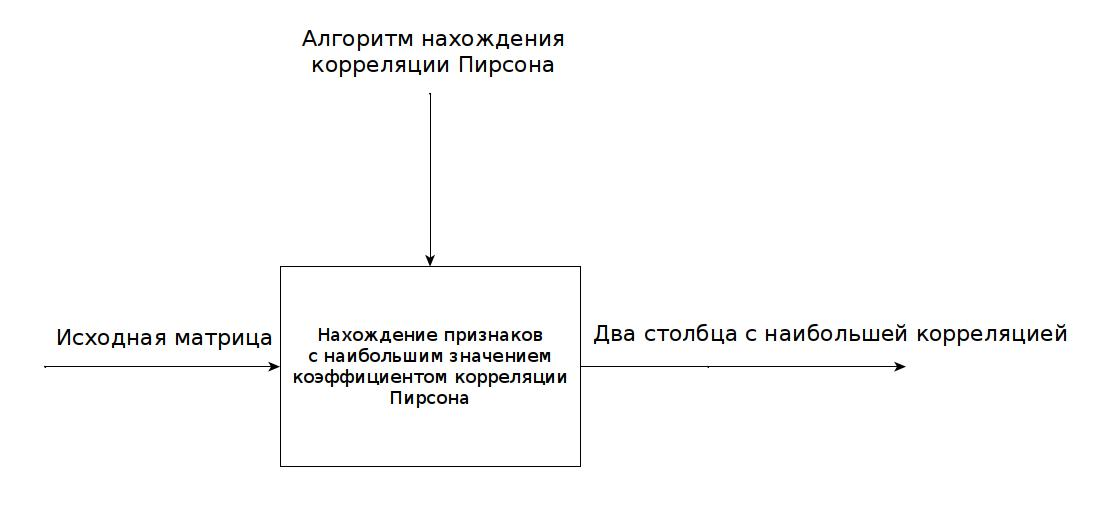
\includegraphics[width=\linewidth]{inc/func.jpg}
	\end{center}
	\caption{Схема классического алгоритма поиска наиболее коррелирующих признаков}
\end{figure}
\FloatBarrier

\section{Схемы алгоритмов}
На рисунке 2.2 будет приведена схема реализации классического алгоритма поиска максимальной корреляции в признаковом пространстве.
На рисунке 2.3 будет приведена схема реализации алгоритма поиска максимальной корреляции в признаковом пространстве с использованием параллельности.

\FloatBarrier
\begin{figure}[hp]
	\label{classic}
	\begin{center}
		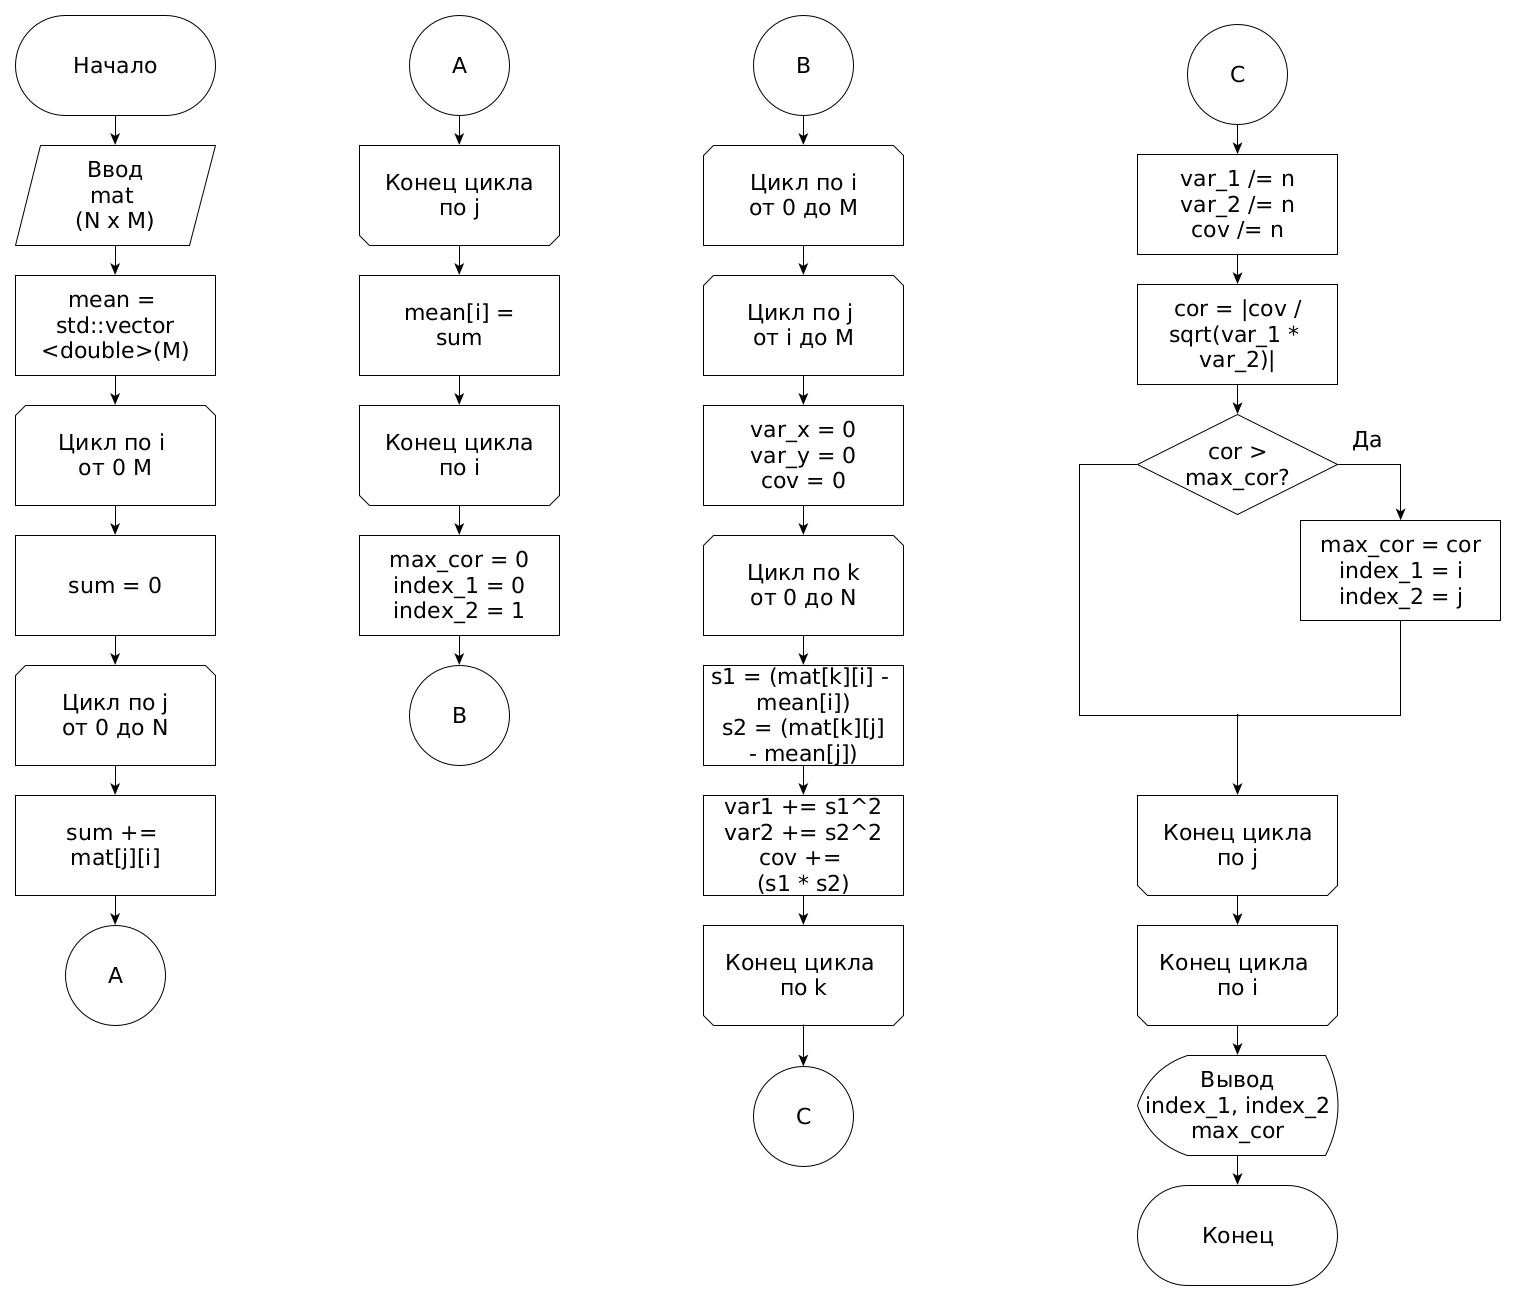
\includegraphics[width=\linewidth]{graph/classic.jpg}
	\end{center}
	\caption{Схема классического алгоритма поиска наиболее коррелирующих признаков}
\end{figure}
\FloatBarrier

\FloatBarrier
\begin{figure}[hp]
	\label{classic}
	\begin{center}
		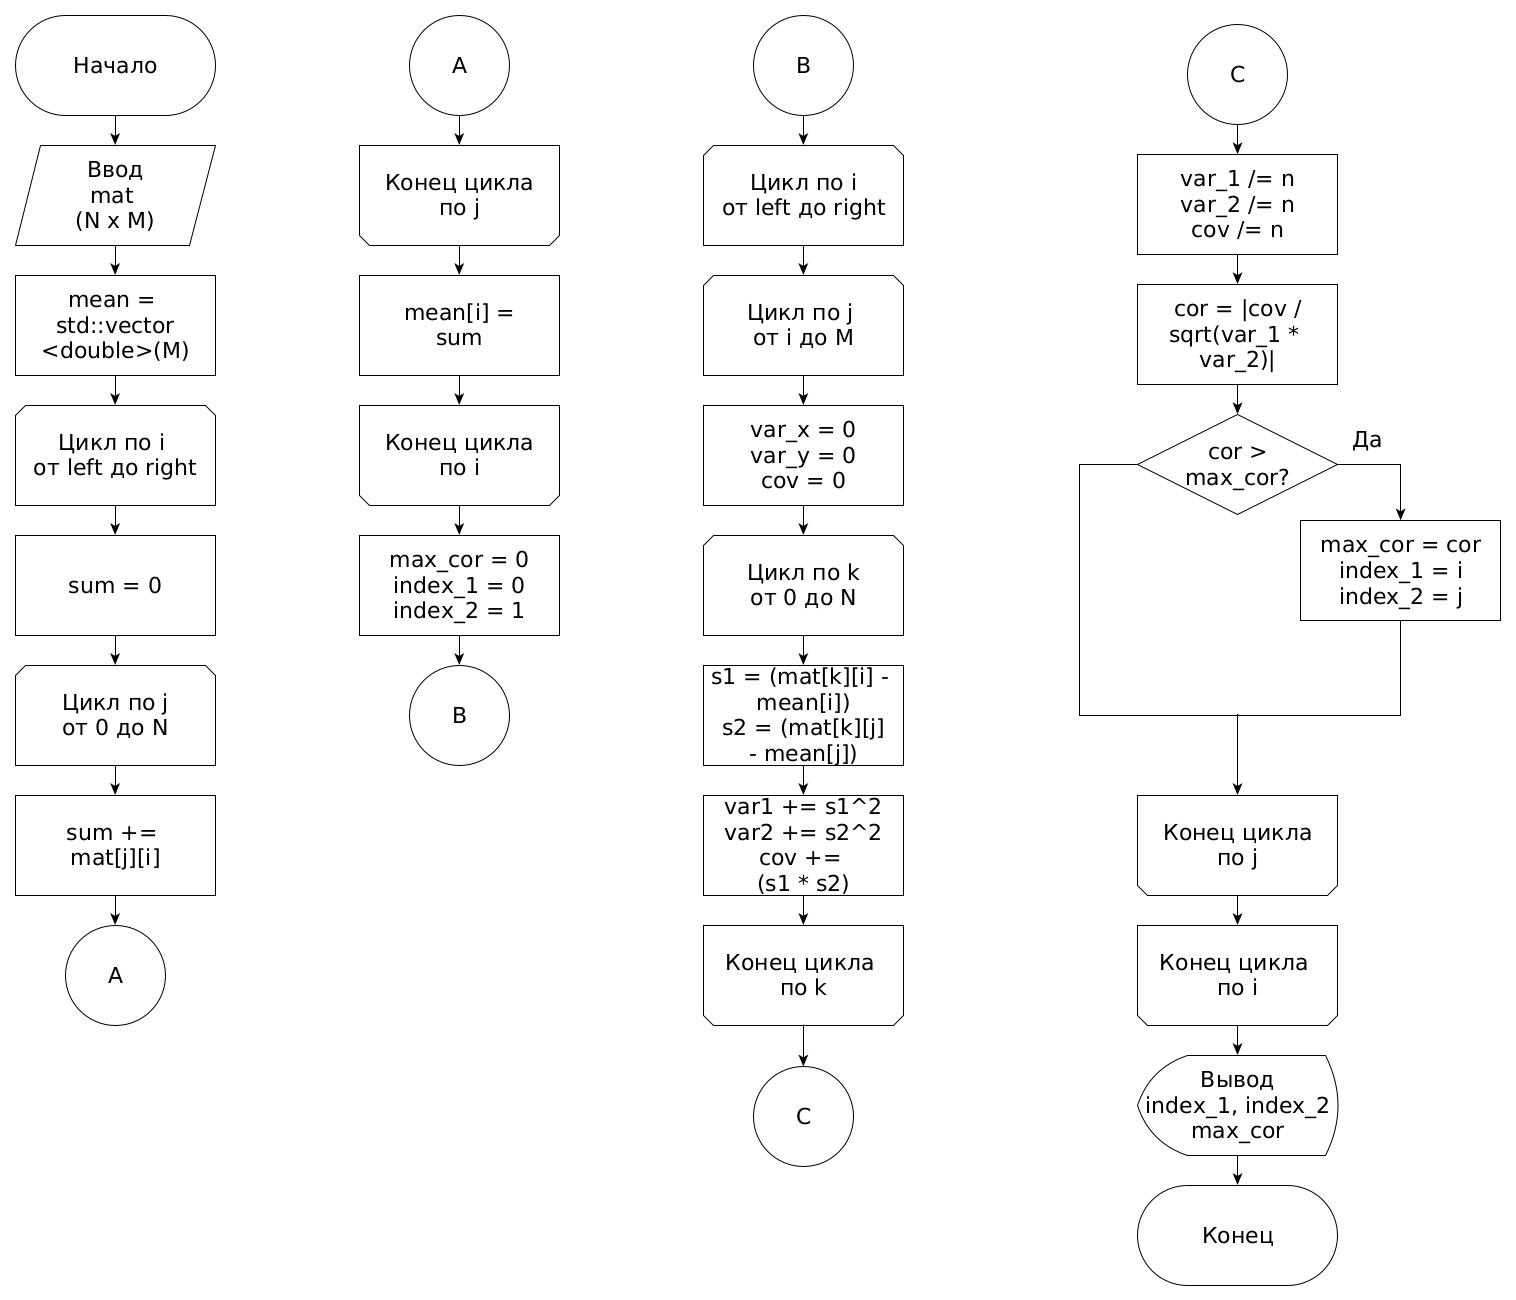
\includegraphics[width=\linewidth]{graph/paral.jpg}
	\end{center}
	\caption{Схема алгоритма поиска наиболее коррелирующих признаков с использованием параллельности}
\end{figure}
\FloatBarrier

Распараллеливание вычислений реализовано благодаря добавлению двух новых переменных {\ttfamily left} и {\ttfamily right}, которые указывают на диапазон строк, которые необходимо рассчитать.


\section{Типы данных для алгоритмов}
Тестирование алгоритмов будет производиться на вещественных числах, 
которые могут быть и отрицательными, и равны нулю. Несмотря на это,
сами реализации алгоритмов универсальны и предназначены для любых численных типов данных.

Размер матрицы может быть произвольным из тех, что допустимы по требованиям ко вводу.

\section{Способ тестирования}
Тестирование программы будет произодиться методом чёрного ящика.
Такой подход выбран, так как от реализаций алгоритмов требуется в первую
очередь правильность работы.
Сама по себе реализация не требует тестировки, так как в точности
повторяет теоретические принципы, сформированные в аналитическом
разделе.

В качестве классов эквивалентности были выбраны следующие сущности:
\begin{itemize}
	\item матрица состоит из двух столбцов;
	\item матрица состоит из двух строк и нескольких столбцов;
	\item между двумя столбцами матрицы прослеживается явная линейная зависимость;
	\item между двумя столбцами матрицы прослеживается явная отрицательная линейная зависимость;
	\item матрица состоит из случайных значений;
\end{itemize}

Для корректного сравнения требуется для каждой реализации умножения матриц
сравнить полученный на выходе результат с эталонным. Для этого будет использоваться библиотека numpy,
то есть предварительно эталонное значение для каждой матрицы будет рассчитано.

\section{Проектирование работы потоков}
В разрабатываемом ПО предполагается, что один из потоков является основным.
Он будет раздавать задания остальным потоком, после этого ждать выполнения каждым потоком задачи.
Так как параллельность выполняется в двух местах, то основной поток будет раздавать задания два раза.

На рисунке 2.4 представлена схематичная временная диаграмма работы потоков программы на примере
8-поточного алгоритма.

\FloatBarrier
\begin{figure}[hp]
	\label{classic}
	\begin{center}
		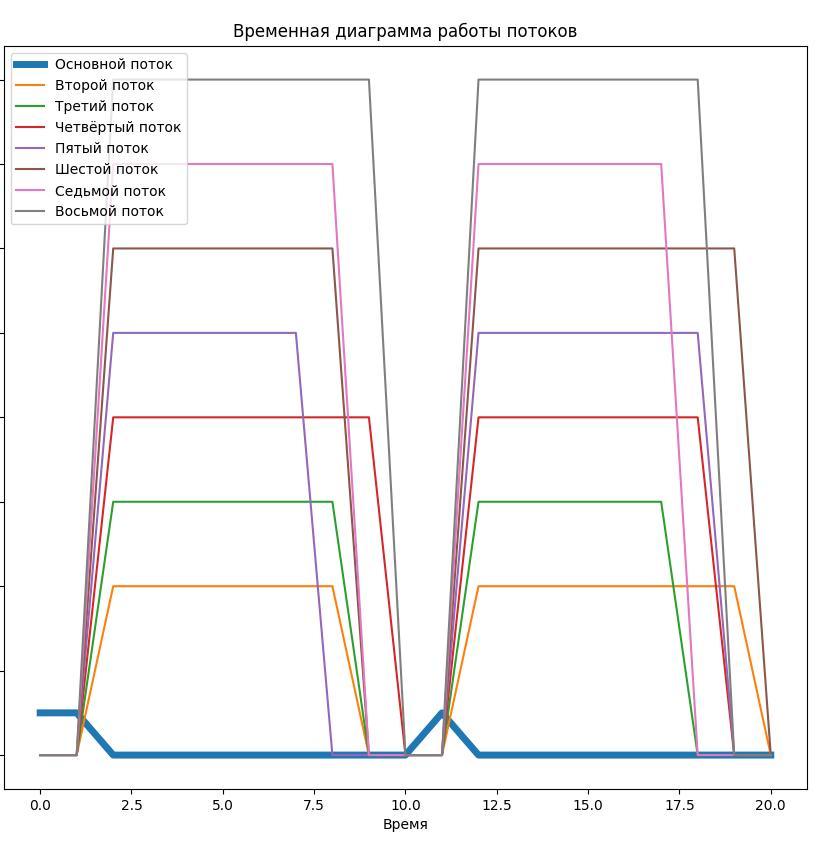
\includegraphics[width=\linewidth]{inc/threads.jpg}
	\end{center}
	\caption{Временная диаграмма работы потоков программы}
\end{figure}
\FloatBarrier

Основной поток после выдачи заданий другим потокам не будет предпринимать никаких действий,
пока все потоки не закончат выполнение своего задания.

Из этого можно сделать вывод, что в случае работы 2-поточного алгоритма, один поток будет основным,
а ещё один поток будет выполнять один все действия, поэтому время работы будет схоже с временем работы
классического алгоритма.

Также для доступа к переменной глобального максимума будет использоваться мьютекс.

\section{Вывод}
Были приведены требования к ПО, схемы реализации алгоритмов.
Были определен способ тестирования алгоритмов.